\documentclass[letterpaper, oneside, 11pt]{book}
\usepackage[left=1in, right=1in, top=0.75in]{geometry}
\usepackage[svgnames]{xcolor}
\usepackage{float}
\usepackage{graphicx}
\usepackage{setspace}
\usepackage{acronym}
\usepackage[sfdefault]{roboto}
\usepackage{xcolor}
\usepackage{sectsty}
\usepackage[colorlinks=true, linkcolor=gray]{hyperref}
\usepackage[utf8]{inputenc}
\usepackage{hyperref}
\definecolor{MyBlue}{rgb}{0.03, 0.27, 0.49}
\chapterfont{\color{MyBlue}}
\sectionfont{\color{MyBlue}}
\subsectionfont{\color{MyBlue}}

\begin{document}
%%========================================================================
\begin{titlepage}
	\raggedleft
	\begin{figure}[H]
	\centering
		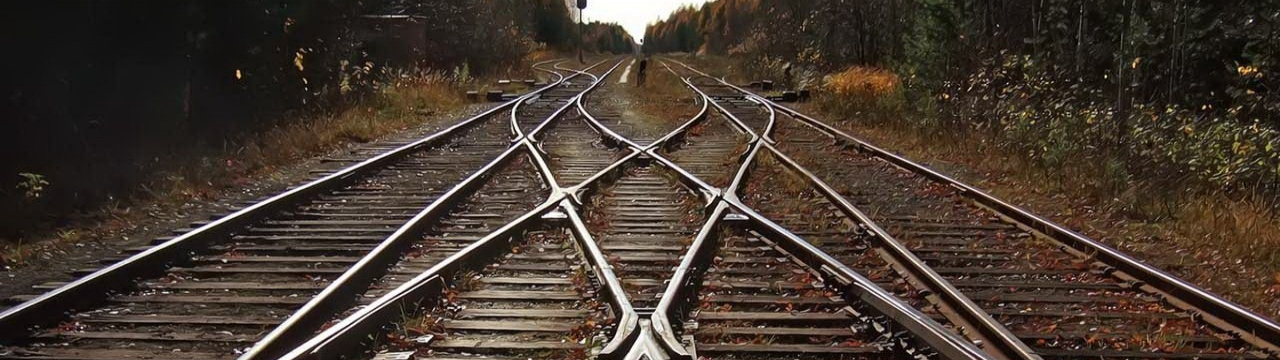
\includegraphics[scale=1.53]{railway_track.jpg}
	\label{fig:track}
\end{figure}
	\vspace*{0.167\textheight}
	\textbf{\LARGE System Design and Implementation}\\[\baselineskip]
    \textbf{\textcolor{MyBlue}{\Huge R\Large ailway \Huge A\Large dministration and \Huge I\Large nformation \Huge L\Large ogical \Huge S\Large ystem}}\\[\baselineskip]
	{\Large \textit{RAILS for Model Railroads}}
	\vfill
    \vspace*{\baselineskip}
	{\small David Bristow}

	{\small Version 2.0.0}
	
	{\small Jan 18, 2023}
	\vspace*{3\baselineskip}
\end{titlepage}
%%========================================================================
\tableofcontents
%% copyright notice
%%========================================================================
\chapter{Microcontrollers for RAILS}
\section{Introduction}
\gls{rails} is a software model and implementation of an automated system to assist the model railroader achieve realism in the operation of a model railroad.
There are four user interface \gls{spa} that provide different aspects of rails they are:
\begin{itemize}
  \item \gls{rsrm} allows the user to match a rfid tag to a rollingstock's road name and number;
  \item \gls{mrim} allows the user to create, update and delete model railroad assets, such as rolling stock;
  \item \gls{mppm} allows the user to enter information about their projects and purchases; and
  \item \gls{mrlm} allows the user to enter information about their layout and control elements of it.
\end{itemize}
\section{RSRM Components}
The implementation of \gls{rsrm} consists of the following micro-services components:
\begin{itemize}
\item \gls{rfid} Controller is a micro-controller that processes \gls{rfid} tags obtained from a \gls{rfid} reader and then publishes \gls{iot} messages to the \gls{mqtt} Broker;
\item \gls{mqtt} Broker is responsible for receiving \gls{rfid} and micro info messages, filtering them, posting to designated topics and sending messages to clients subscribing to topics. The subscribers and publishers bridge the \gls{mqtt} elements with the GUI applications. The broker handles \gls{iot} messages;
\item \gls{isrs} subscribes to \gls{rfid} messages and pushes them via a web-socket to the rsm component;
\item \gls{isms} that subscribes to micro controller startup and heartbeat messages, updating the micros collection via \gls{rlds};
\item \gls{rlds} provides \gls{rest} access to model railroad layout collections including micros;
\item \gls{rids} provides \gls{rest} access to railroad inventory collections including rollingstock;
\item MongoDB a NoSQL database program that stores data records as documents which are gathered in collections. A database stores one or more collections of documents;
\item \gls{mr} Data is the document repository, used by MongoDB, to store complete collections of items such as rollingstock, industries (producers and consumers), track elements, turnouts, projects, purchases, etc. in support of \gls{rails}; and
\item \gls{rsrm} is the \gls{spa} that allows a user to match a \gls{rfid} tag to a rollingstock's road name and number.
\end{itemize}
Figure \ref{fig:rsms-ms-components} depicts the micro-services used to create the rolling stock \gls{rfid} management subsystem.

\begin{figure}[H]
	\centering
		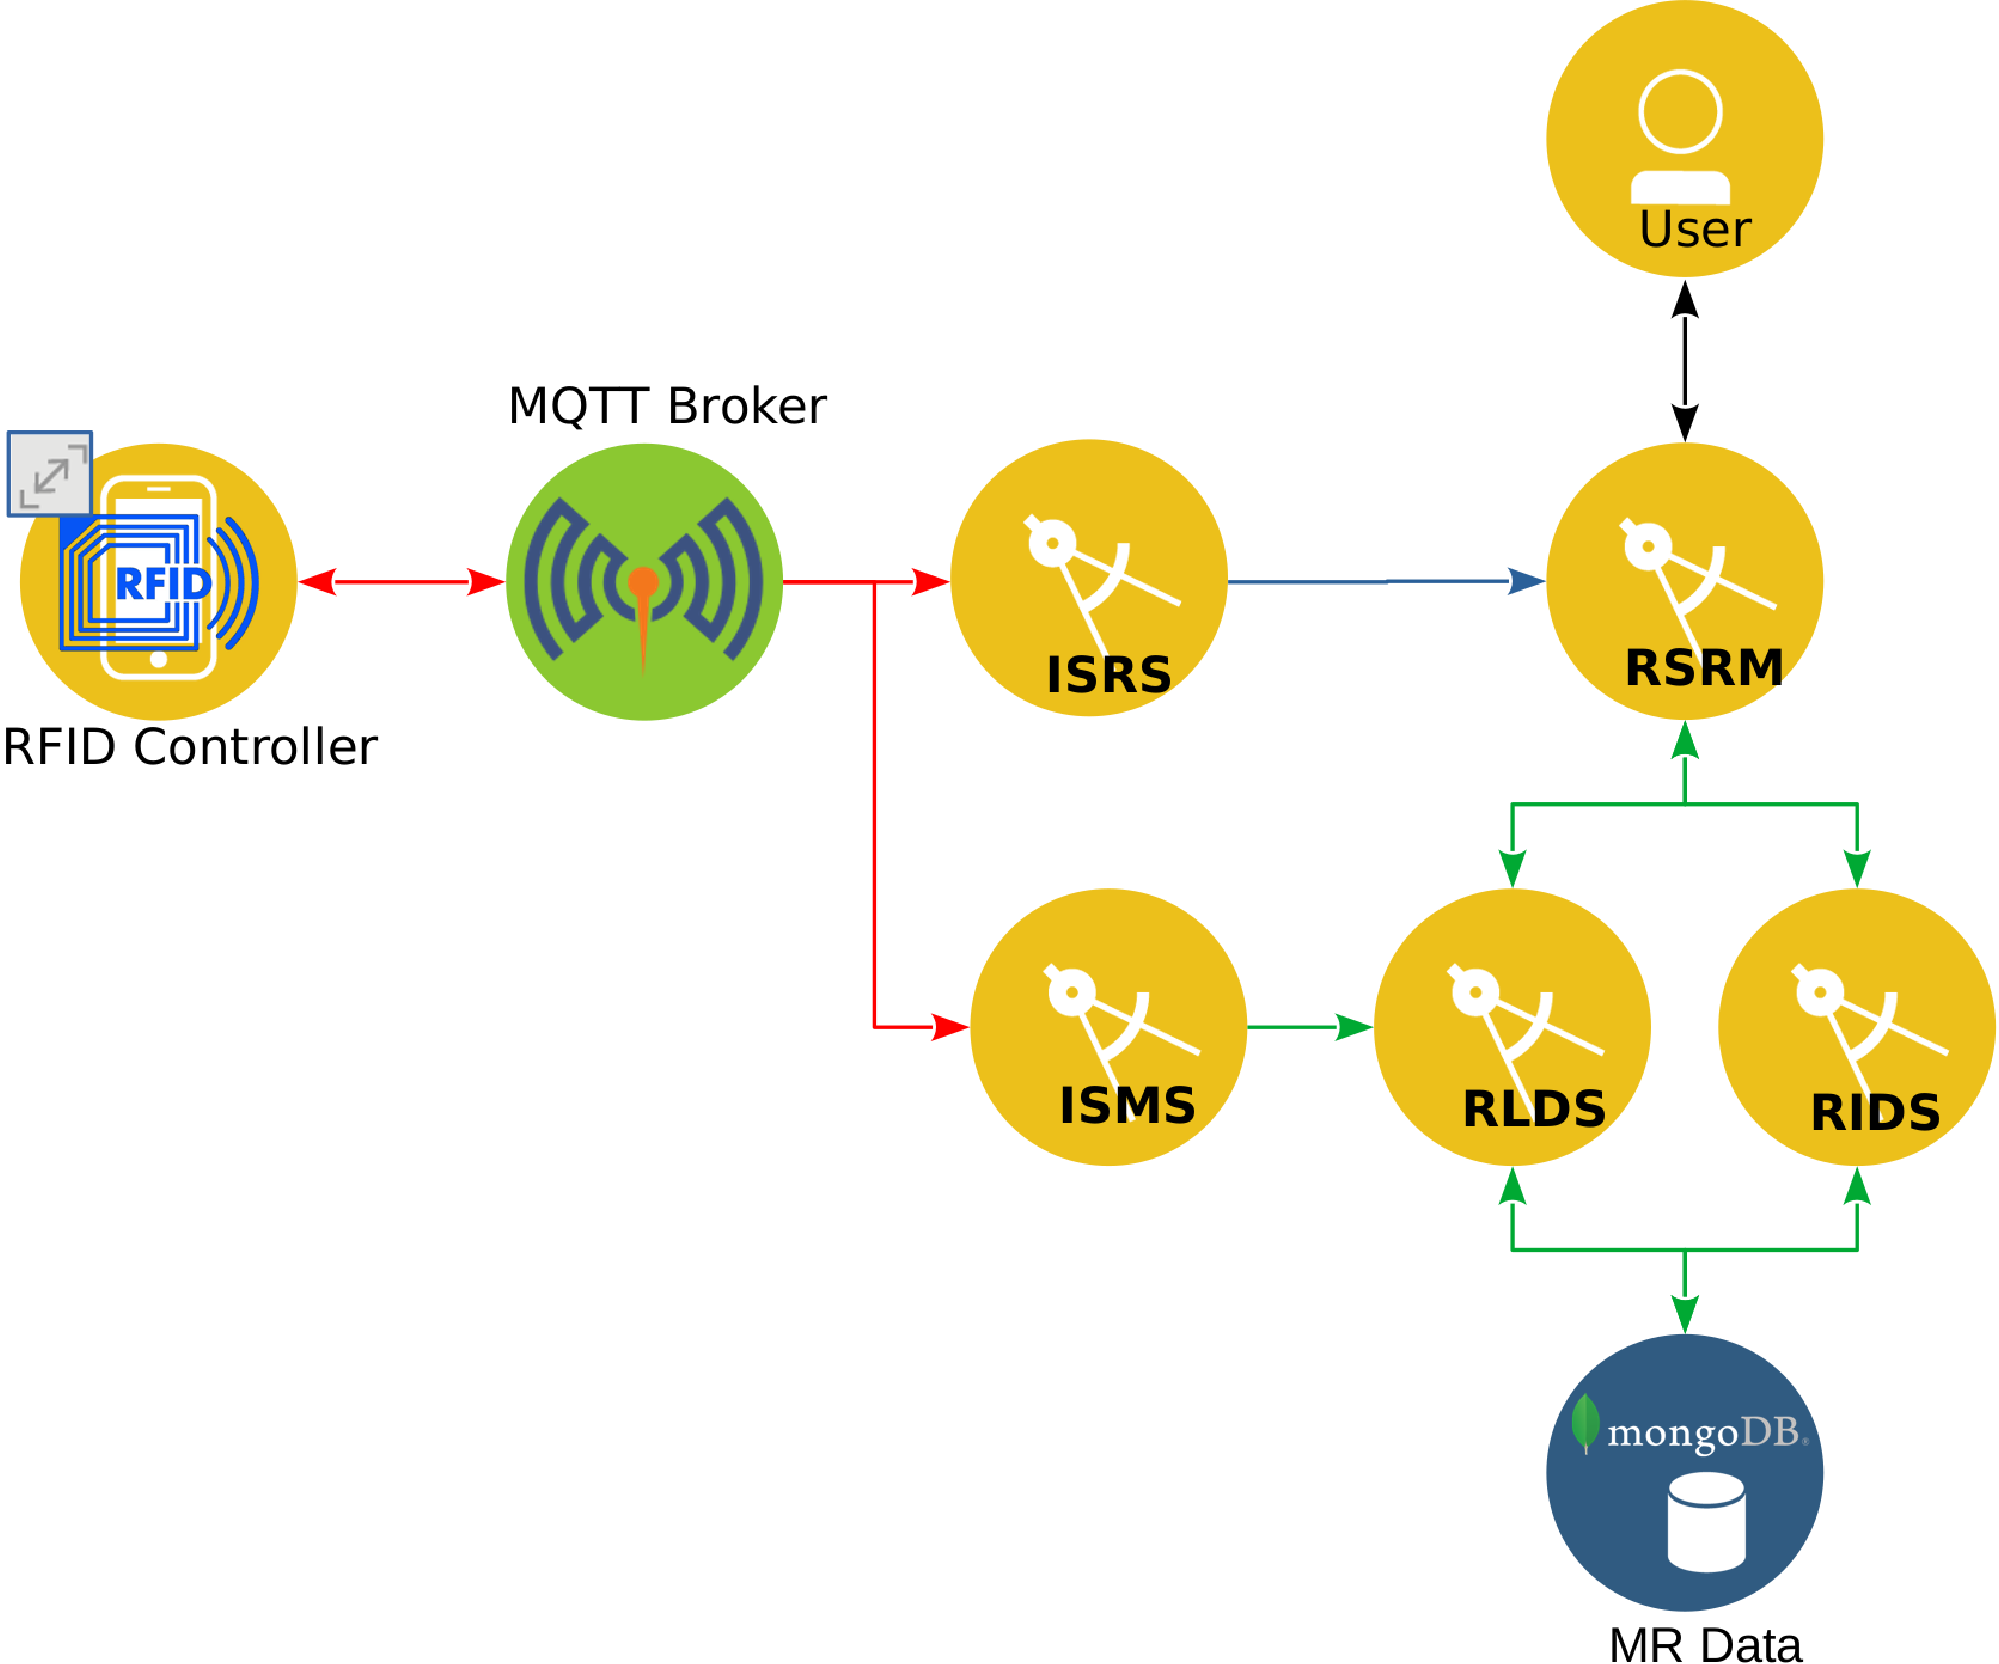
\includegraphics[scale=0.15]{../Images/rsms_microservices.png}
	\caption{Microservices Components}
	\label{fig:rsms-ms-components}
\end{figure}

Three system components that make up this subsystem:
\begin{itemize}
\item \gls{rfid} Controller is a micro-controller that processes \gls{rfid} tags obtained from a \gls{rfid} reader and then publishes \gls{iot} messages to the \gls{mqtt} Broker;
\item Network is a \gls{tcpip} communication medium that connects the \gls{rfid} Controller, \gls{mqtt} Broker and \gls{rsrm} components; and
\item Host is a computer that runs the \gls{mqtt} Broker and other \gls{rsrm} micro-services components.
\end{itemize}
Figure \ref{fig:rsms-system} depicts the systems components used to create the rolling stock \gls{rfid} management subsystem.

\begin{figure}[H]
	\centering
		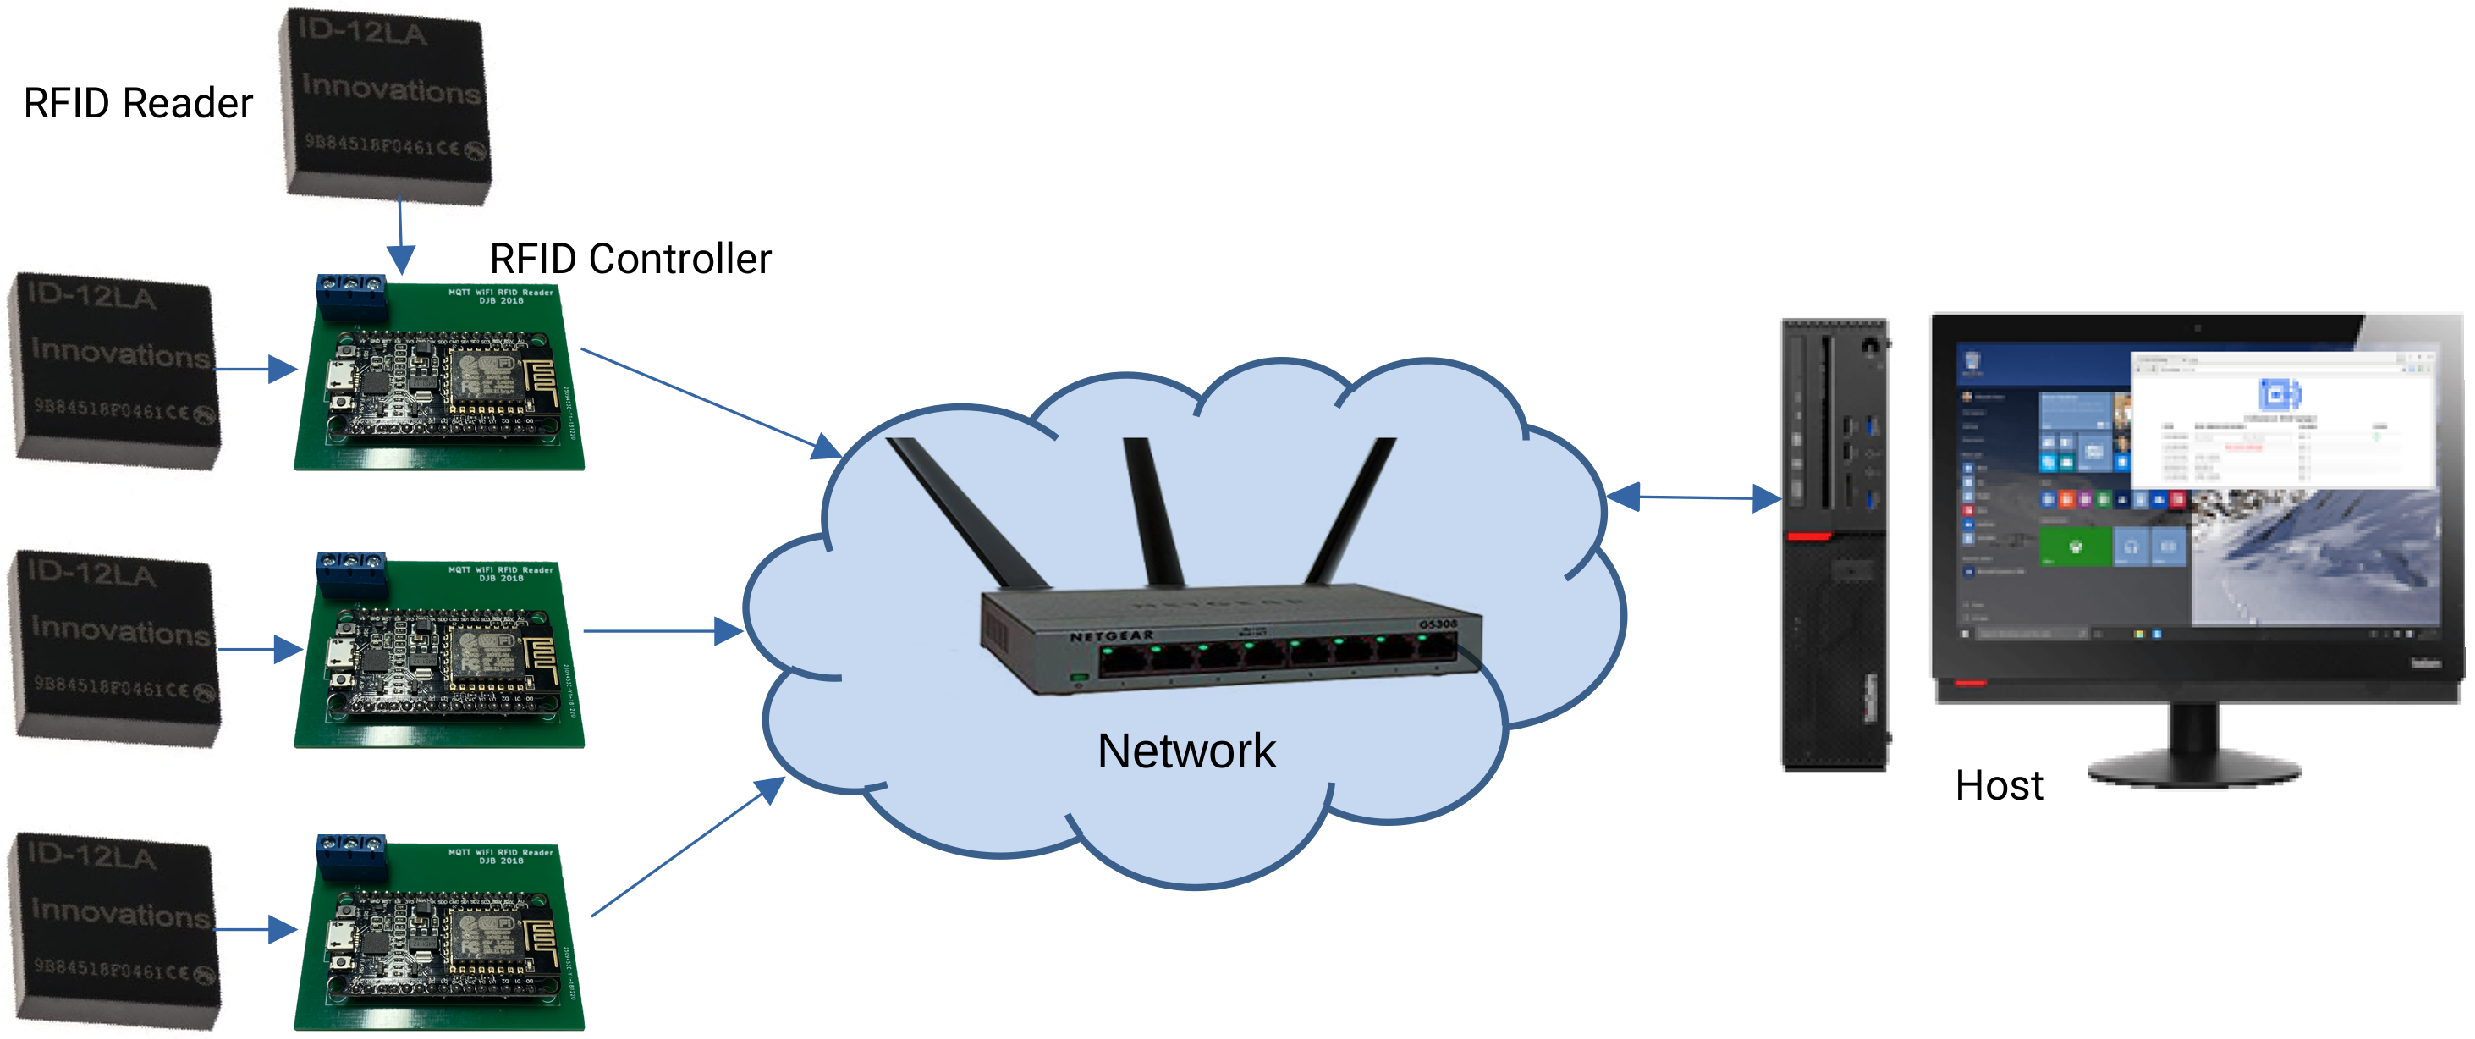
\includegraphics[scale=0.15]{../Images/rsms_system.png}
	\caption{RSMS System Components}
	\label{fig:rsms-system}
\end{figure}

\section{MRLM System Components}

Figure \ref{fig:mrlm-ms-components} depicts the micro-services used to create the \gls{mrlm} subsystem and figure \ref{fig:turnout-system} depicts it's logical architecture.

\begin{figure}[H]
	\centering
		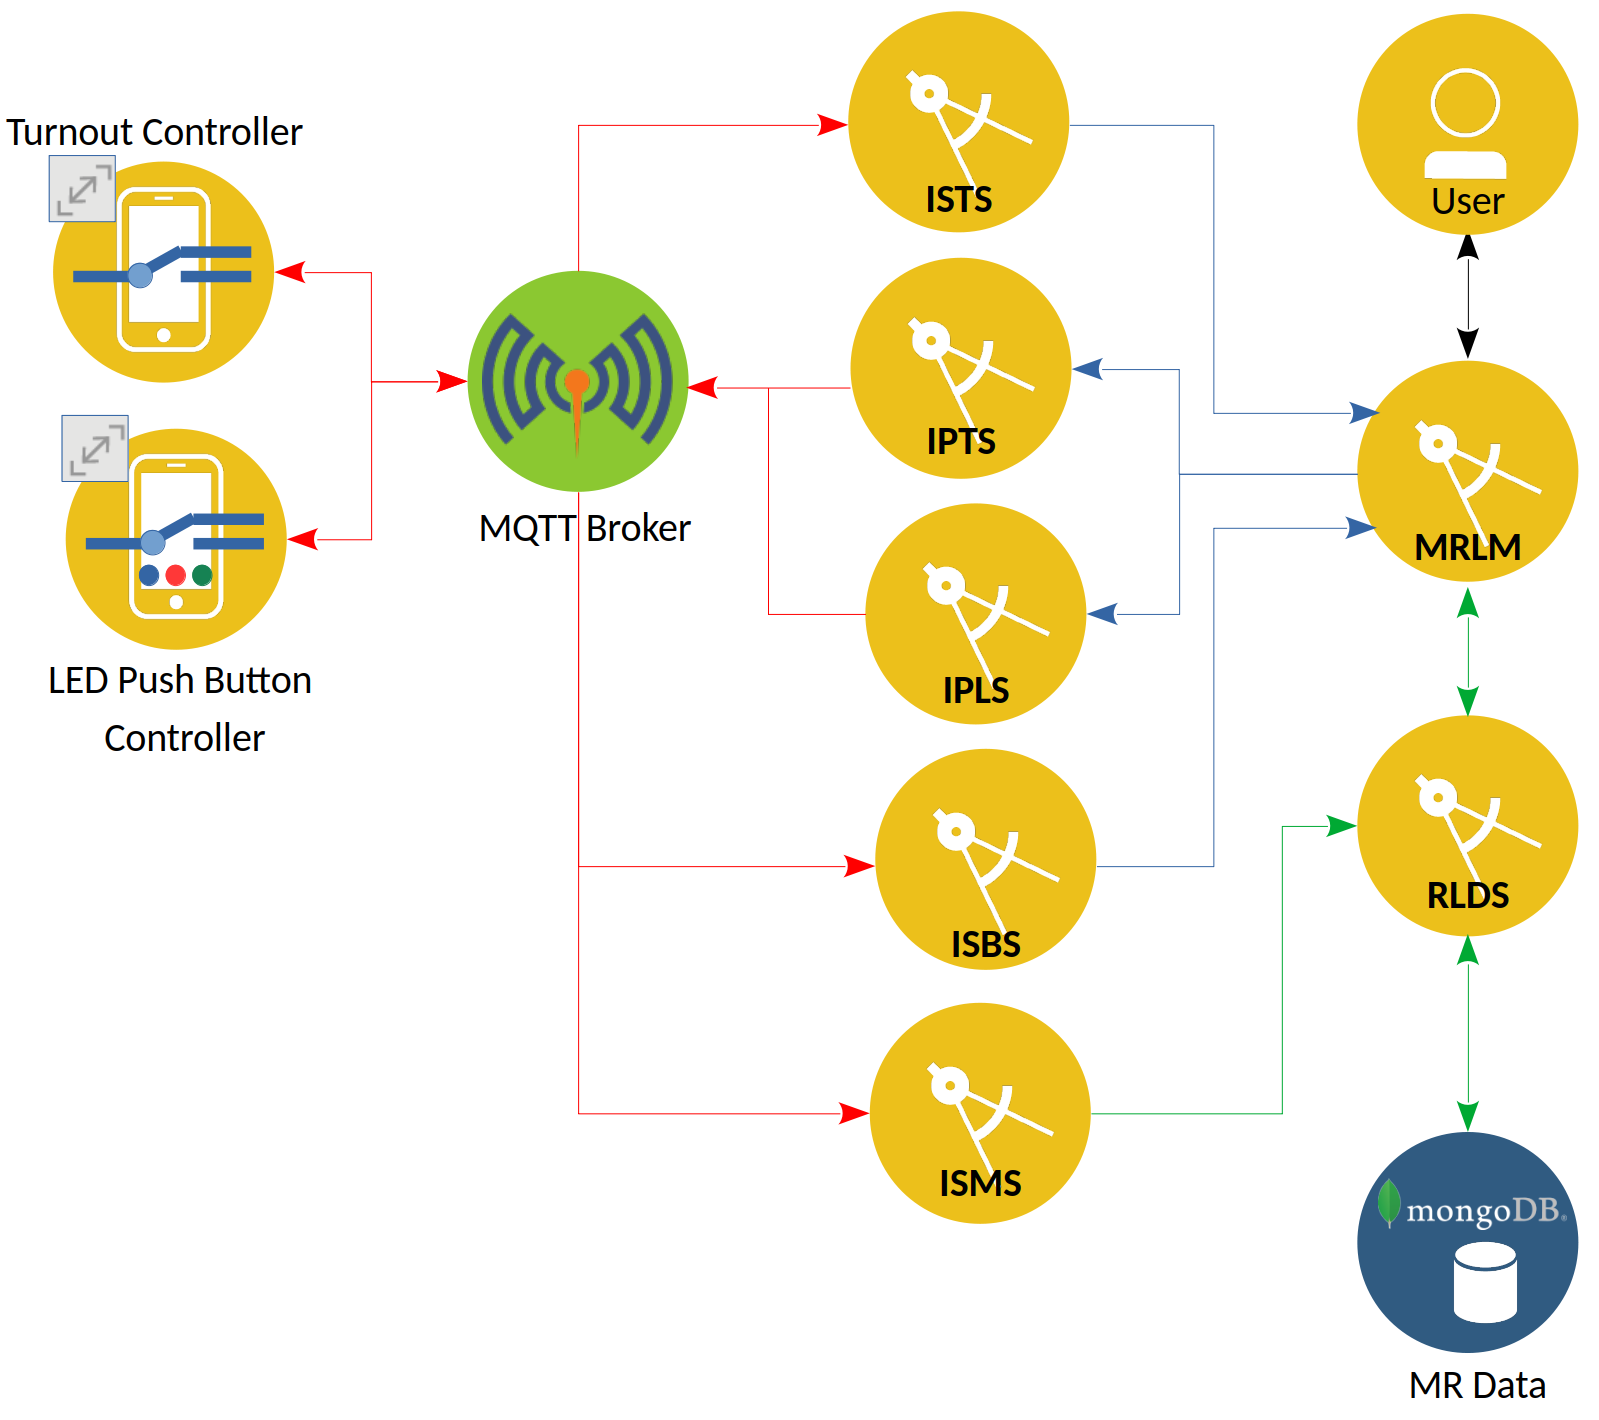
\includegraphics[scale=0.2]{../Images/mrlm_microservices.png}
	\caption{Microservices Components}
	\label{fig:mrlm-ms-components}
\end{figure}


\begin{figure}[H]
	\centering
		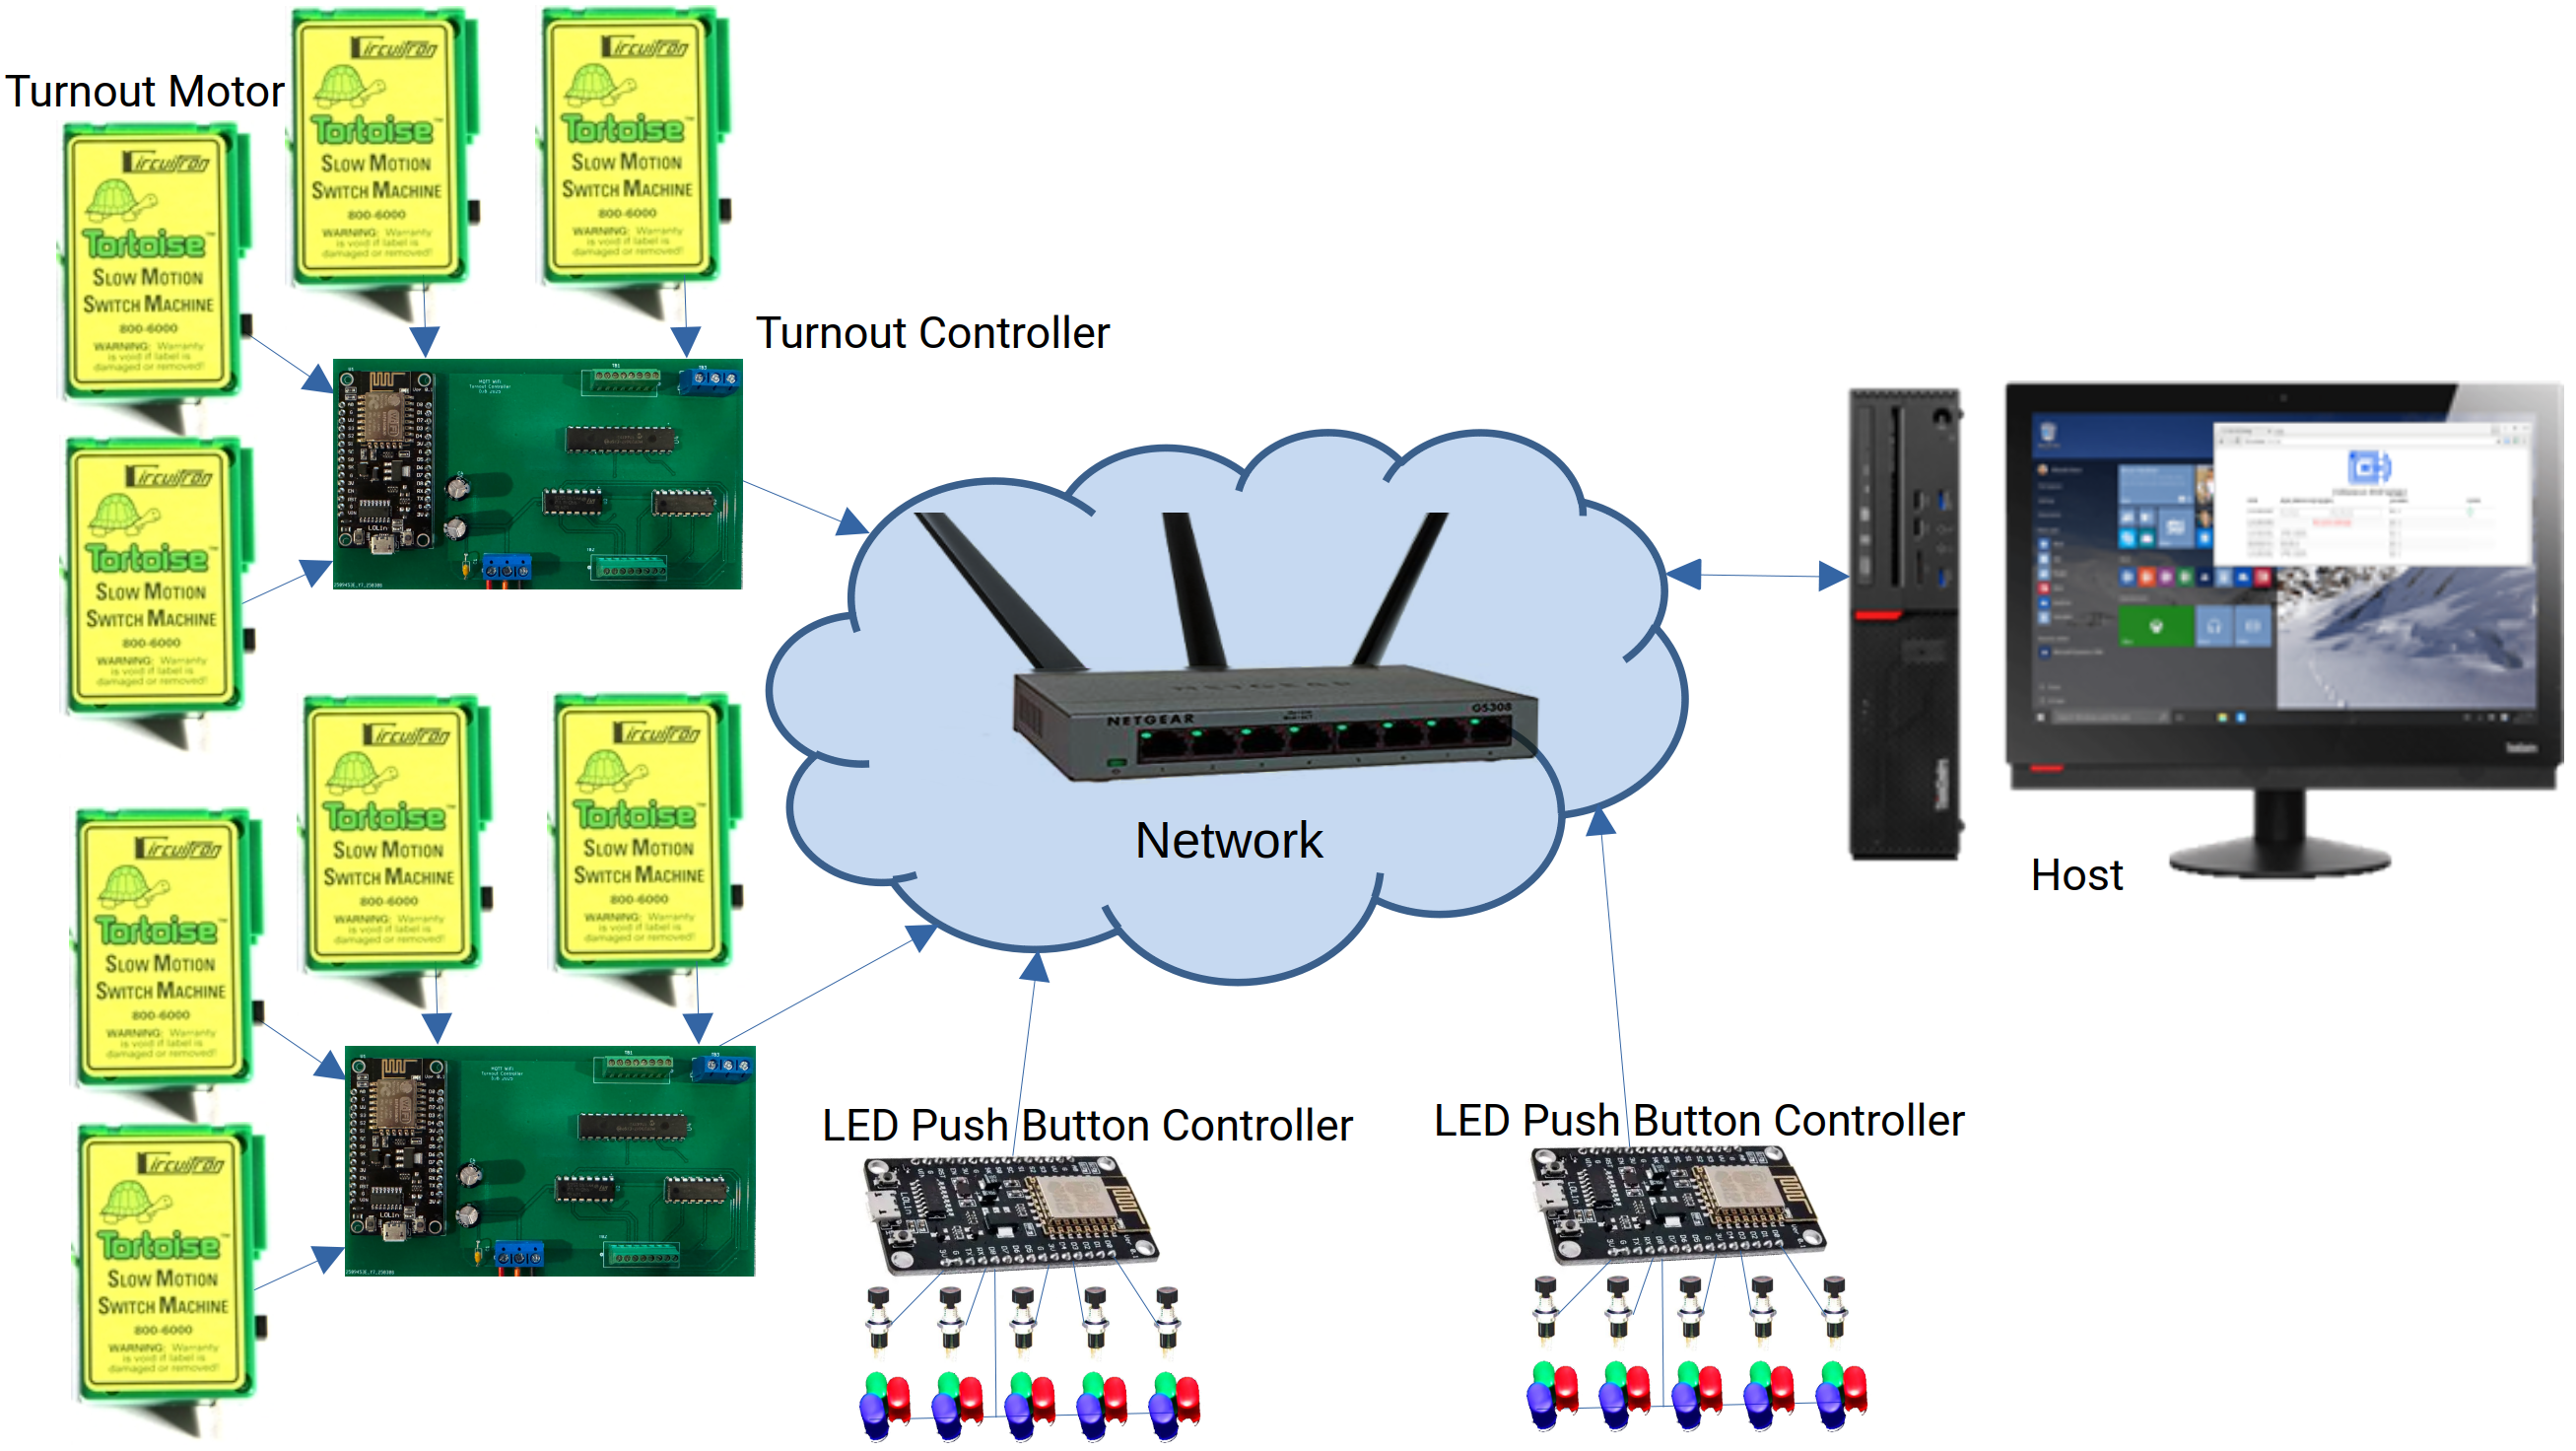
\includegraphics[scale=0.2]{../Images/mrlm_system.png}
	\caption{MRLM System Components}
	\label{fig:turnout-system}
\end{figure}

\chapter{Use Case Survey Model}
A use case survey model is a method of identifying and documenting the specific tasks and activities that a particular group of users (such as modelers or operators) performs with a product or system. The goal of a use case survey is to understand how the users interact with the product or system, and to identify opportunities for improvement or potential areas of confusion or frustration. The survey typically includes a series of questions that ask the users to describe their tasks and activities, as well as any problems or issues they have encountered. The results of the survey are then analyzed to identify patterns and trends, which can be used to inform design and development decisions.\vspace{5mm} \\
Use cases are used in software development to describe how a system or product should behave in response to certain inputs or events. They provide a clear and detailed understanding of the requirements for a system, and serve as a communication tool between developers, stakeholders and users. These are depicted as ellipses in the survey model.\vspace{5mm} \\
Some of the key benefits of using use cases include:
\begin{itemize}
  \item They help to identify the specific functional requirements of a system, which can be used to guide the design and development process.
  \item Use cases provide a clear and detailed description of how a system should behave in response to different inputs, which can be used to test the system and ensure that it meets the requirements.
  \item Use cases can be used to identify and document the different types of users and their specific needs, which can be used to inform user-centered design decisions.
  \item They provide a clear and consistent way to communicate the requirements of a system to different stakeholders, including developers, business analysts, and project managers.
  \item Use cases can be used to identify potential risks and problems early in the development process, which can help to minimize the impact of these issues on the overall project.
\end{itemize}
In use case modeling, an actor is a person or system that interacts with the system being developed. Actors represent the external entities that interact with the system in order to achieve a specific goal or accomplish a specific task.\vspace{5mm} \\
Each actor is typically defined by a set of characteristics, such as their role, responsibilities, and the specific tasks or activities they perform with the system. Actors can be either human users or other systems that interact with the system being developed.\vspace{5mm} \\
In the use case diagram, actors (human) are represented by stick figures and actors (systems) are represented by subsystem packages. Actors are usually connected to the use cases they interact with by an arrow.\vspace{5mm} \\
Use case actors are important because they help to identify the different types of users or systems that interact with the system, which can be used to inform user-centered design decisions. Actors also help to identify the specific requirements of the system, which can be used to guide the development process and ensure that the final product meets the needs of all stakeholders.\vspace{5mm} \\
Figure \ref{fig:use-case} depicts the use case survey model used to design and develop \ac{RAILS}.
In figure \ref{fig:use-case} the line color:
\begin{itemize}
  \item blue indicates the actor use case relationship
  \item orange indicates an inheritance relationship where the open arrow is the inherited.
  \item purple indicates a uses relationship where the open arrow is the used use case.
\end{itemize}
\begin{figure}
	\centering
		\includegraphics[scale=0.55]{use-case.eps}
	\caption{Use Case Survey Model}
	\label{fig:use-case}
\end{figure}
\section{Actors}
\subsection{Human Actors}
\begin{itemize}
  \item Dispatcher is responsible to develop an operating session plan in which rolling stock is assigned to consists and those consists are routed and scheduled.
  \item Model Railroad Manager is responsible to establish and maintain railroad network; rolling stock inventory; defining \ac{DCC} parameters for appropriate rolling stock; industries and their cargo types; schedule rolling stock and railroad network components for maintenance; initial operating states for all turnouts, signals and \ac{DCC} components.
  \item Model Railroad Modeler is responsible to create, modify, and dispose of model railroad assets.
  \item Session Operator is responsible to execute part or all an operating session plan, outside of the rail yard, using the system and the \ac{DCC} Subsystem.
  \item Session Supervisor is responsible to supervise the execution of part or all an operating session plan by the Session Operators and Yard Masters. This person may also function as a Session Operator.
  \item Yard Master is responsible to execute part of an operating session plan, by assembling the consists inside the rail yard, using the system and the \ac{DCC} Subsystem.
\end{itemize}
\subsection{Subsystem Actors}
\begin{itemize}
  \item \ac{DCC} Subsystem is responsible to transmit messages to rolling stock equipped with \ac{DCC} receiver/controller, as commanded by the system and to warn the system of possible malfunctions.
  \item Sensor Subsystem is responsible to detect the presence of rolling stock in a railroad network block/segment and provide notification to the system.
  \item Signal Subsystem is responsible to change the state of specified signals located on the rail network as commanded by the system.
  \item Turnout Subsystem is responsible to indicate the state of turnouts on the rail network; change the state of turnouts as commanded by the system; and indicate operators’ action to change the state of turnouts.
  \item Panel Subsystem is responsible for displaying status information about turnouts and providing operator input to change turnout position.
\end{itemize}
\section{Use Cases}
\begin{itemize}
  \item Configure Industries is responsible to establish and maintain the Industry database, allowing the manager to add, modify or delete industries, simulate production/consumption of goods as cargo, and inform the dispatcher of industry cargo requirements.
  \item Control Model Railroad is responsible to assist the operator in managing the execution of an operating session plan. By:
\begin{itemize}
  \item automatically executing the parts of an operating session plan selected by the operator for regular scheduled trains by commanding the Signal, Turnout and \ac{DCC} subsystems; and
  \item assisting the operator executing parts of an operating session plan by commanding the Signal, Turnout and \ac{DCC} subsystems.
\end{itemize}
  \item Configure Maintenance is responsible to establish and maintain the maintenance database, allowing the manager to schedule rolling stock or railroad network components maintenance, simulate component failures, and warn the dispatcher of needed maintenance
  \item Configure Network is responsible to establish and maintain the railroad network database, allowing the manager to add, modify or delete railroad network components, and to initialize the Signal and Turnout Subsystems automatically at startup and as requested by the manager.
  \item Configure Rolling Stock is responsible to establish and maintain the rolling stock database, allowing the manager to add, modify or delete rolling stock and inform the dispatcher of the rolling stock attributes.
  \item Develop Operating Session Plan is responsible to assist the dispatcher in developing an operating session plan.
  \item Dispatch Trains Automatically is responsible for executing the operating session plan autonomously.
  \item Dispatch Trains Manually is reponsible to assist the operators execute the operating session plan.
  \item Shutdown Model Railroad is responsible to bring the system down gracefully ensuring the state be stored so that when the system Startup occurs the system returns to the state when the system was shutdown.
  \item Startup is responsible to bring the system up in either a distributed environment or standalone mode.
  \item Track Model Railroad Assets is responsible to establish and maintain the model railroad asset database, allowing the modeler to add, or modify assets and manage modeling projects.
\end{itemize}

\chapter{Microservices Design Components}
Figure \ref{fig:microarchitecture} shows the microservices components that make up the design of \gls{rails}.

\begin{figure}[H]
	\centering
		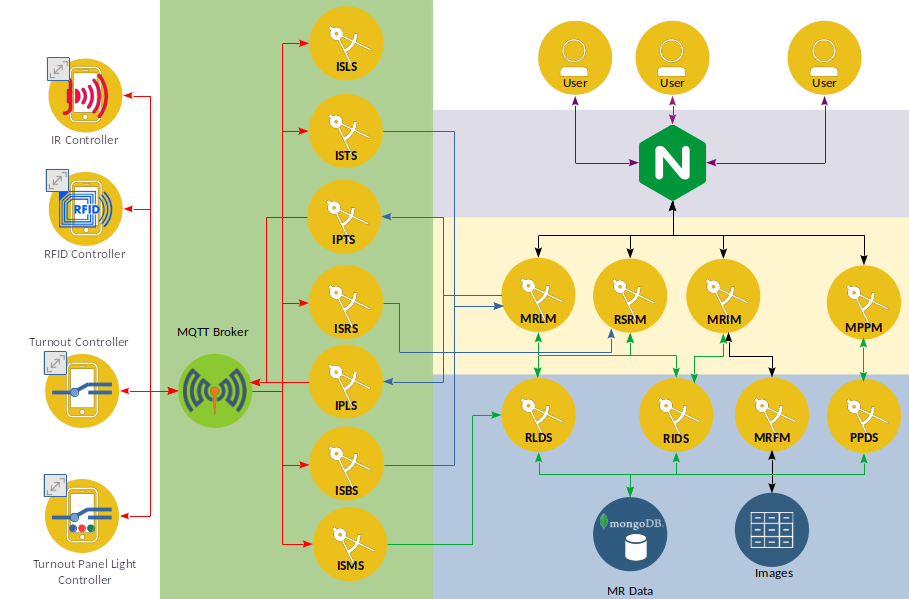
\includegraphics[scale=0.7]{design.png}
	\caption{Microservices Component Architecture}
	\label{fig:microarchitecture}
\end{figure}

The microservices design components are divided into four sets:
\begin{itemize}
  \item \gls{iot} components, which are highlighted with the light green colored background in Figure \ref{fig:microarchitecture}.
  \item \gls{ds} components, which are highlighted with the light blue colored background in Figure \ref{fig:microarchitecture}.
  \item \gls{spa} components, which are highlighted with the buff colored background in Figure \ref{fig:microarchitecture}.
  \item a reverse proxy, which is highlighted with the mauve colored background in Figure \ref{fig:microarchitecture}.
\end{itemize}

\section{\gls{iot} Components}
The components of the \gls{iot} set of design components are subdivided into:
\begin{itemize}
  \item Micro Controllers using the \gls{mqtt} protocol:
\begin{itemize}
  \item \gls{rfid} Controller processes \gls{rfid} tags obtained from a \gls{rfid} reader and then publishes the value
  \item Turnout Controller subscribes to turnout commands then to act on the command to cause the turnout to move. It then publishes the state of the turnout
  \item \gls{ir} Controller (in planning) processes \gls{ir} sensors and publishes their values
\end{itemize}
  \item \gls{mqtt} Broker is the heart of any publish/subscribe protocol, is responsible for receiving messages, posting to designated topics and sending messages to clients subscribing to topics.
  \item The subscribers and publishers bridge the \gls{mqtt} elements with the \gls{gui} applications:
\begin{itemize}
  \item \gls{ipls} publishes turnout panel light commands a Turnout Panel Controller
  \item \gls{ipts} publishes turnout commands to a Turnout Controller
  \item \gls{isbs}  subscribes to push button events and pushes them via a web-socket to the MRLM component
  \item \gls{isls} (in planning) \gls{iot} subscribes to topics that provide location information i.e., \gls{ir} Sensors and \gls{rfid} sensors
  \item \gls{isms} subscribes to micros and adds or updates micros collection in RAILS. It also subscribes to micro heartbeats.
  \item \gls{isrs} subscribes to \gls{rfid} tags and pushes them via a web-socket to the \gls{rsrm} component
  \item \gls{ists} subscribes to turnout switch closures and pushes them via a web-socket to the \gls{mrlm} component
\end{itemize}
\end{itemize}
\section{DS Components}
\gls{ds} consist of all the components that handle and or store the model railroad data:
\begin{itemize}
  \item MR Data – the document repository, MongoDB, to store complete collections of items such as rolling stock, industries (producers and consumers), track elements, turnouts, projects, purchases, etc.
  \item \gls{rids} provides \gls{rest} access to railroad inventory documents
  \item \gls{ppds} provides \gls{rest} access to model railroad projects and purchases documents
  \item \gls{rlds} provides \gls{rest} access to model railroad layout documents
  \item \gls{mrfm} provides the user the ability to upload image files for the use by the \gls{mrim} component
  \item Images is the file store for the images uploaded by \gls{mrfm} component and used by the \gls{mrim} component
\end{itemize}
\section{SPA Components}
\gls{gui} applications that provide user access to RAILS:
\begin{itemize}
  \item \gls{rsrm}, this \gls{spa} allows a user to match a RFID value to a rolling stock road name and number
  \item \gls{mrim}, this \gls{spa} allows a user to create, update and delete model railroad assets, such as rolling stock
  \item \gls{mppm}, this \gls{spa} allows a user to enter information about their projects and purchases
  \item \gls{mrlm}, this \gls{spa} allows a user to enter information about their layout and control elements of it
\end{itemize}
\section{Reverse Proxy}
A server that sits in front of the \gls{spas}, which allows users to access the \gls{spas} from any browser on any \gls{pc} in the network. Using a reverse proxy offers a wide range of practical benefits — from performance and scalability to security and maintainability. However, the principal use of the reverse proxy server in \gls{rails} is to allow multiple browsers on different \gls{pcs} in the same \gls{lan} to view any of the \gls{spas}.


\chapter{IoT Design}

In software architecture, the publish/subscribe pattern is a messaging pattern where senders of messages (publishers), do not program the messages to be sent directly to specific receivers (subscribers), but instead categorize published messages into topics without knowledge of which subscribers, if any, there may be. Subscribers express interest in one or more topics, and only receive messages that are of interest, without knowledge of which publishers, if any, there are. This pattern decouples senders and receivers, allowing for greater scalability and a more dynamic communication environment.\vspace{5mm} \\
Eclipse Mosquitto is an open-source message broker software that implements the \ac{MQTT} protocol, a standard for publish/subscribe messaging for the \ac{IoT}. Mosquitto provides a lightweight way for IoT devices to communicate with each other, allowing them to publish and subscribe to messages on topics. With Mosquitto, devices can publish information, such as sensor readings or status updates, to the message broker and receive updates from other devices. Mosquitto helps to facilitate efficient and effective communication between \ac{IoT} devices in a scalable manner.\vspace{5mm} \\
Table \ref{iot-table} identifies functions excuted by microcontrollers and the \ac{IoT} messaging attributes.\vspace{5mm} \\

\begin{table}[!ht]
    \begin{center}
    \begin{tabular}{|l|l|l|l|}
    \hline
        \textbf{Micro Function} & \textbf{Pub/Sub} & \textbf{Topic} & \textbf{Message} \\ \hline
        RFID Reader & Pub & sensors/rfid & RFID \\ \hline
        Turnout Contacts & Pub & sensors/toc & Turnout\\ \hline
        Turnout Panel Push Button & Pub & sensors/pb & \\ \hline
        Heartbeat & Pub & micros & Micro Info\\ \hline
        Turnout & Sub & acts/to/cntrlr id &  \\ \hline
        Turnout Panel Light & Sub & acts/tpl/cntrlr id &\\ \hline
        Micro Info & Pub & micros & Micro Info\\ \hline
    \end{tabular}
    \caption{\label{iot-table}IoT Micro Function Table}
    \end{center}
\end{table}

Figure \ref{fig:iotdesign} depicts the flow of \ac{MQTT} messages through the \ac{MQTT} broker from and to microservices components.

\begin{figure}[H]
	\centering
		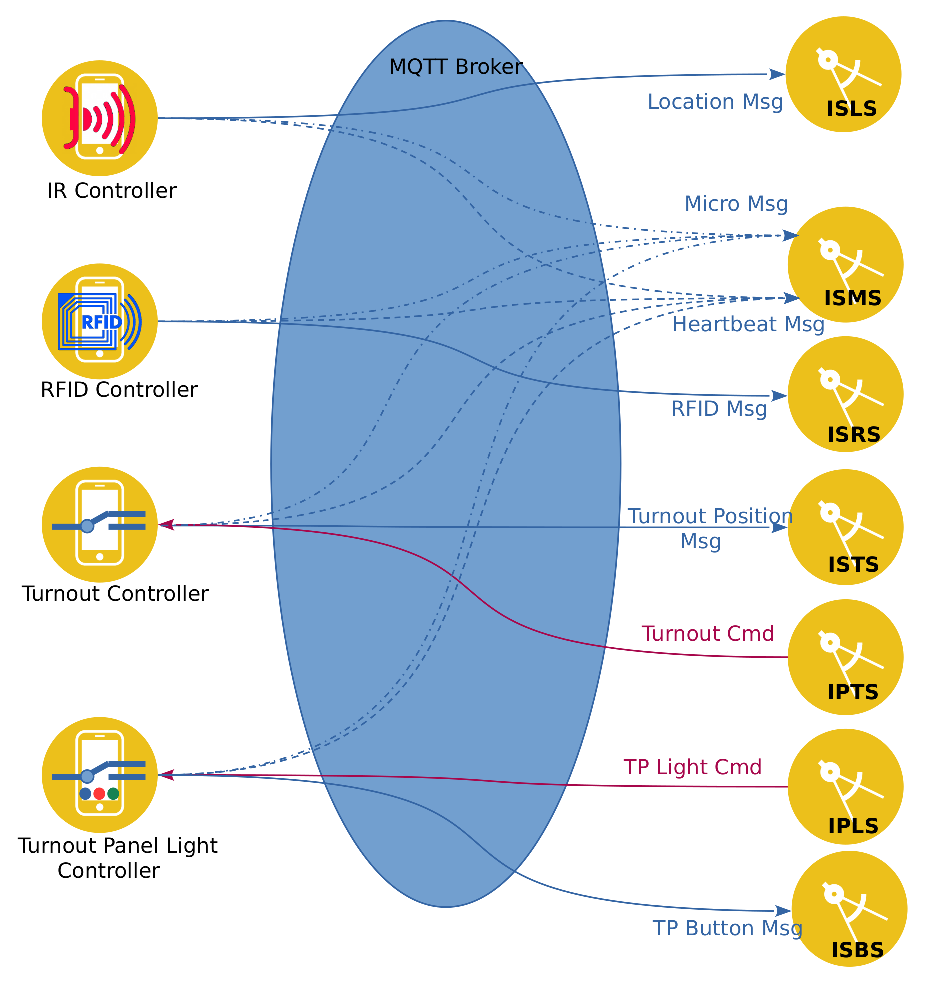
\includegraphics[scale=0.7]{mqtt-v7.eps}
	\caption{IoT Design}
	\label{fig:iotdesign}
\end{figure}

\section{Message Definitions}
\begin{itemize}
\item \ac{RFID} message format: \{“et”:“epoch time",”sensor”:”sensor id“,”rfid”:”rfid tag value“\}
\begin{itemize}
\item example \{"et":"1590463450","sensor":"rfidRdr01","reader":"1","rfid":"1C0044CF23"\}
\end{itemize}
\item\{“et”:”epoch time“,”cntrlr”:”turnout controller id“,”to”:”turnout number“,”state”:”THROWN|CLOSED|ERROR“\}
\item\{“et”:”epoch time“,”cntrlr”:”turnout panel controller id“,”pb”:”push button number“\} 
\item\{“cntrlr”:”turnout controller id“,”to”:”turnout number“,”cmd”:”THROW|CLOSE|STATUS“\}
\item\{“cntrlr”:”turnout panel controller id“,”tpl”:”light number“,”color”:”RED|GREEN|BLUE“,”type”:”BUTTON”\}
\item Micro Info message format: \{“et”:”epoch time“,”sensor”:”sensor id“,"msgType":"initial|heartbeat","ip":"Address of Micro"\}
\begin{itemize}
\item 'heartbeat' example: \{"et":"1590462747","sensor":"rfidRdr01","msgType":"heartbeat"\} 
\item 'initial' example: \{"et":"1590462747","sensor":"rfidRdr01","msgType":"initial","ip":"192.168.0.19"\}
\end{itemize}
\end{itemize}

\chapter{Software Development Environment}

\section{Visual Studio Code}
A development environment, also known as an \ac{IDE}, is a software tool or a set of tools that provides a comprehensive environment for developers to create, edit, test, and debug software applications. It encompasses various components, features, and functionalities that aid in the software development process.\vspace{5mm} \\
A development environment typically includes the following key elements:
\begin{itemize}
  \item Code Editor: A code editor is the central component of a development environment. It provides a text editor with features like syntax highlighting, code completion, code navigation, and formatting. It allows developers to write and modify code efficiently.
  \item Compiler/Interpreter: A development environment often includes a compiler or interpreter specific to the programming language being used. It translates the written code into executable or interpretable form.
  \item Build Tools: Build tools automate the process of compiling, linking, and packaging software applications. They help in managing dependencies, generating binaries, and performing other build-related tasks.
  \item Debugging Tools: Debugging tools enable developers to identify and fix issues in their code. They provide features like breakpoints, stepping through code, inspecting variables, and tracking program execution flow.
  \item Version Control Integration: Many development environments integrate with version control systems like Git, allowing developers to manage and track changes in their codebase, collaborate with others, and handle branching and merging.
  \item Project Management: Development environments often offer project management features to organize and manage multiple files and resources within a project. They may include features like project templates, file navigation, and project-specific settings.
  \item Testing Framework Integration: Some development environments integrate with testing frameworks, making it easier to write and run unit tests, perform automated testing, and generate test reports.
  \item Documentation Support: Development environments may provide features to assist in documenting code, such as auto-generating documentation, code commenting support, and integration with documentation generation tools.
  \item Integration with External Tools and Libraries: A good development environment allows seamless integration with external tools, libraries, and frameworks specific to the chosen programming language or platform. This makes it easier to utilize third-party libraries and leverage existing ecosystem resources.
  \item Customization and Extension: Development environments often offer extensibility through plugins, extensions, or a package management system. This allows developers to enhance the functionality of the environment by adding new features or integrating with additional tools.
\end{itemize}
Overall, a development environment provides a unified and streamlined workflow for software development, bringing together essential tools and features needed to write, test, and debug code effectively. It aims to improve productivity, code quality, and collaboration among developers.\vspace{5mm} \\
\ac{VS Code} is such an \ac{IDE} that is used to develop and maintain \ac{RAILS}.\vspace{5mm} \\
\ac{VS Code} is developed and maintained by Microsoft and has gained significant popularity among developers worldwide. The following factors and attributes have contributed to the widespread adoption of \ac{VS Code}:
\begin{itemize}
  \item \ac{VS Code} supports many different programming languages, including JavaScript, TypeScript, Python, C++, C\#, Java, and many others. Its flexibility and extensive language support make it appealing to a broad range of developers.
  \item \ac{VS Code} offers excellent support for web development. Its integration with web technologies, such as HTML, CSS, and JavaScript, combined with the availability of various extensions, makes it a preferred choice for building web applications.
  \item \ac{VS Code} is an open-source project with an active community of contributors. This open nature encourages collaboration, fosters innovation, and enables developers to extend and customize the editor to suit their specific needs.
  \item \ac{VS Code} is available for Windows, macOS, and Linux, making it accessible to developers across different operating systems. Its consistent user interface and features across platforms contribute to its popularity.
  \item \ac{VS Code} is known for its speed and performance. It is lightweight compared to many other \acp{IDE}, making it quick to start up and responsive even when working with large codebases.
  \item \ac{VS Code} provides a rich ecosystem of extensions, allowing developers to enhance their development environment. The marketplace offers a wide range of extensions for various programming languages, frameworks, and tools, enabling developers to customize their setup and improve their productivity.
  \item \ac{VS Code} includes an integrated terminal, eliminating the need to switch between the editor and an external command-line interface. This seamless integration enhances the development workflow, allowing developers to execute commands, run scripts, and interact with their projects without leaving the editor.
  \item \ac{VS Code} Code offers strong integration with version control systems like Git. It provides a built-in version control interface, allowing developers to manage their code repositories, track changes, and resolve conflicts directly within the editor.
  \item The \ac{VS Code} community is active and vibrant. Developers can find help, tutorials, and resources through official documentation, community forums, and online platforms. This active support system contributes to the growth and adoption of the editor.
  \item Microsoft and the open-source community continue to actively develop and improve \ac{VS Code}. Regular updates introduce new features, performance enhancements, and bug fixes, ensuring that the editor remains up-to-date and meets the evolving needs of developers.
  \item \ac{VS Code} provides a rich and extensible \ac{IDE} experience with features like code highlighting, autocompletion, code navigation, and debugging.
  \item \ac{VS Code} has excellent integration with Git, enabling version control management within the editor. The Git functions commit, pull, push, and resolve merge conflicts are provided by \ac{VS Code}.
\end{itemize}
\ac{VS Code} with PlatformIO is a powerful combination for developing embedded systems and \ac{IoT} projects. PlatformIO is an open-source ecosystem that provides a unified development platform for different microcontrollers, development boards, and frameworks. When used together, Visual Studio Code and PlatformIO offer a range of features and capabilities for embedded development. Here are some things that can be done with \ac{VS Code} and PlatformIO:
\begin{itemize}
  \item PlatformIO supports various development platforms, including Arduino, ESP-IDF, mbed, STM32, and many more. It is easy to switch between different platforms and frameworks within \ac{VS Code}.
  \item PlatformIO integrates with a vast library repository, making it easy to search, install, and manage libraries for projects. It simplifies the process of adding external libraries to the projects code.
  \item PlatformIO provides a powerful build system that handles the compilation and linking of the project's code. It supports different build configurations and allows the user to customize the build process.
  \item PlatformIO includes a serial monitor feature that allows the user to communicate with the user's embedded device over a serial interface. The user can send and receive data, monitor logs, and troubleshoot issues.
\end{itemize}
\ac{VS Code} provides excellent support for Node.js and web development, including frameworks like Vue 3. 
\begin{itemize}
  \item \ac{VS Code} offers excellent support for Vue development. With the "Volar" extension installed, it provides features like IntelliSense, syntax highlighting, code snippets, and error checking for Vue templates, JavaScript, and CSS.
  \item \ac{VS Code} offers a range of features to enhance the JavaScript code editing experience. It provides syntax highlighting, code formatting, and auto-completion out of the box.
  \item \ac{VS Code} has built-in support for code formatting and linting. It is possible to configure any project's formatting and linting rules using tools like Prettier and ESLint.
  \item \ac{VS Code} has an integrated terminal that allows the ability to run Node.js commands and scripts without switching to an external terminal.
\end{itemize}
\section{MQTTX}
MQTTX is a free and open-source \ac{MQTT} client tool that provides a graphical user interface (GUI) for working with \ac{MQTT}. It is designed to facilitate the testing, debugging, and monitoring of \ac{MQTT}-based applications. \ac{MQTT} is a lightweight messaging protocol commonly used in \ac{IoT} and other applications that require efficient, reliable, and real-time communication between devices or clients and a server.\vspace{5mm} \\
MQTTX offers the following features:
\begin{itemize}
  \item MQTTX connects to \ac{MQTT} brokers (servers) and manages multiple connections simultaneously. It supports connecting to brokers using various authentication methods, such as username/password or certificates.
  \item With MQTTX, enables the user to publish messages to \ac{MQTT} topics and subscribe to topics to receive messages. It provides an intuitive interface to define topic names, payloads, and QoS (Quality of Service) levels for both publishing and subscribing.
  \item MQTTX maintains a message history, which allows the user to review and analyze previously sent and received messages. It provides a payload preview feature to visualize the content of messages, helping the user understand the data being transmitted.
  \item MQTTX displays a topic tree that provides a hierarchical view of MQTT topics. This helps the user navigate through the topics and easily subscribe to or unsubscribe from specific topics. It also supports filtering messages based on topic patterns, making it easier to manage and monitor specific topics of interest.
  \item MQTTX includes built-in tools for encoding and decoding payload data in various formats, such as JSON, Base64, and Hex. This is useful for analyzing and manipulating payload data during testing and debugging.
  \item  MQTTX supports secure communication using TLS/SSL encryption. It allows the user to configure and connect to MQTT brokers that require secure connections, providing an additional layer of data protection.
\end{itemize}
MQTTX is available for different operating systems, including Windows, macOS, and Linux. Its user-friendly interface and feature-rich environment make it a valuable tool for developers working with MQTT-based applications, enabling efficient testing, debugging, and monitoring of MQTT communications.
\section{MongoDB Compass}
MongoDB Compass is a graphical user interface \ac{GUI} tool provided by MongoDB Inc. It is designed to simplify the process of working with MongoDB databases. Compass allows users to interact with their MongoDB databases visually, providing an intuitive way to explore, analyze, and manipulate data.\vspace{5mm} \\
Some key features of MongoDB Compass include:
\begin{itemize}
  \item Compass provides an easy-to-use interface for navigating and exploring MongoDB databases and collections. Users can view documents, query data, and understand the structure of their data through a graphical representation.
  \item Compass includes visual query and aggregation builders that allow users to construct MongoDB queries and aggregations without writing any code. This feature helps users who may not be familiar with the MongoDB query language to easily interact with their data.
  \item Compass provides real-time monitoring and performance analysis tools to help users optimize their MongoDB deployments. It offers insights into query execution times, index usage, and other performance metrics, allowing users to identify and address performance bottlenecks.
  \item Compass allows users to create, modify, and delete indexes on their MongoDB collections. It provides recommendations for index creation based on query patterns and can help users improve the performance of their database queries.
  \item Compass includes a schema validation feature that enables users to define rules for the structure and content of their MongoDB documents. It helps maintain data integrity by validating incoming documents against predefined schemas.
  \item Compass supports importing and exporting data to and from MongoDB databases. Users can import data from various file formats, such as JSON or CSV, and export data to these formats as well.
\end{itemize}
Overall, MongoDB Compass is a powerful tool that simplifies the management and interaction with MongoDB databases, providing a visual and user-friendly interface for developers, database administrators, and data analysts.
\section{Git \& GitHub}
Git is a distributed \ac{VCS} used for tracking changes in source code during software development. It was created by Linus Torvalds, the creator of the Linux operating system, in 2005. Git allows multiple developers to collaborate on a project by providing a mechanism to manage and merge their code changes efficiently.\vspace{5mm} \\
GitHub is a web-based hosting service and collaboration platform for Git repositories. It provides a centralized location where developers can store, manage, and collaborate on their Git repositories. GitHub offers a variety of features and tools that enhance the functionality of Git and facilitate collaboration among developers and teams.\vspace{5mm} \\
Microsoft acquired GitHub in June 2018 in a deal worth \$7.5 billion. Following the acquisition, GitHub continues to operate as an independent platform, maintaining its brand, services, and user base while also benefiting from Microsoft's resources and support.\vspace{5mm} \\
GitHub provides the following features:
\begin{itemize}
  \item GitHub allows users to host their Git repositories on its servers. Developers can create repositories to store their code and version history.
  \item GitHub promotes social collaboration and networking among developers. Users can follow other developers, star and fork repositories, and contribute to open-source projects.
  \item GitHub includes an issue tracking system where users can create, assign, and track issues related to their projects. Issues can be used to report bugs, suggest enhancements, or discuss project-related topics.
  \item GitHub provides features such as wikis, project boards, and discussions to help teams collaborate effectively. Wikis allow for documentation and knowledge sharing, project boards help manage tasks and workflows, and discussions provide a platform for team communication.
  \item GitHub Pages is a feature that enables users to host static websites directly from their repositories. It simplifies the process of publishing and sharing web content.
\end{itemize}
GitHub offers both free and paid plans, with additional features and storage available in the paid tiers. It has become a popular choice for individual developers, open-source projects, and large organizations due to its user-friendly interface, strong community, and extensive features for code collaboration and project management.
\section{Docker}
Docker is an open-source platform that enables developers to automate the deployment, scaling, and management of applications using containerization. Containers are lightweight, isolated environments that encapsulate an application and all its dependencies, including libraries, frameworks, and other runtime components. Docker allows the user to package an application into a container image, which can then be run consistently across different environments, such as development, testing, and production.\vspace{5mm} \\
Docker provides the following features:
\begin{itemize}
  \item Docker containers are portable and can run on any system that supports Docker, regardless of the underlying operating system or infrastructure. This eliminates the "works on my machine" problem and ensures consistent behavior across different environments.
  \item Containers provide a high level of isolation, ensuring that applications and their dependencies are encapsulated and do not interfere with each other. This isolation improves security, as well as prevents conflicts between different software components.
  \item Docker containers are lightweight and share the host system's operating system kernel. This means they require fewer resources compared to traditional virtual machines (VMs). Multiple containers can run on the same host without significant performance overhead.
  \item Docker makes it easy to scale applications horizontally by running multiple instances of containers across different hosts or a cluster of machines. This enables efficient utilization of resources and helps handle increased workload demands.
  \item Docker allows versioning of container images, making it easier to track changes and roll back to a previous version if needed. This simplifies the deployment and update process, reducing the risk of application downtime.
  \item Docker has a large and active community, resulting in a vast ecosystem of pre-built container images available from Docker Hub and other registries. These images can be easily pulled and used as a base for building and deploying applications, saving development time.
\end{itemize}

 \href{https://www.emqx.com/en/blog/the-easiest-guide-to-getting-started-with-mqtt}{MQTT Protocol Explained: The Basics and a Quick Tutorial}

\href{https://mqttx.app/?utm_source=mqttx&utm_medium=referral&utm_campaign=logo-to-homepage}{MQTTX}

 \href{https://code.visualstudio.com/docs}{Getting Started with Visual Studio Code}

 \href{https://www.docker.com/}{Docker}




%%========================================================================
\backmatter

\chapter{Acronyms}
\begin{acronym}
\acro{API}{Application Program Interface}
\acro{CLI}{command-line interface}
\acro{DCC}{Digital Command and Control}
\acro{DS}{Data Services}
\acro{EJB}{Enterprise Java Bean}
\acro{GUI}{Graphic User Interface}
\acro{IDE}{Integrated Development Environment}
\acro{I/O}{input/output}
\acro{IR}{Infrared}
\acro{IoT}{Internet of Things}
\acro{IPLS}{IoT Publisher Turnout Panel Light Services}
\acro{IPTS}{IoT Publisher Turnout Services}
\acro{ISBS}{IoT Subscriber Turnout Panel Button Services}
\acro{ISLS}{IoT Subscriber Location Services}
\acro{ISMS}{IoT Subscriber Micro-controller Services}
\acro{ISRS}{IoT Subscriber RFID Services}
\acro{ISTS}{IoT Subscriber Turnout Services}
\acro{JEE}{Java Enterprise Edition}
\acro{JSF}{JavaServer Faces}
\acro{MQTT}{Message Queuing Telemetry Transport}
\acro{MRFM}{Model Railroad File Manager}
\acro{MRIM}{Model Railroad Inventory Manager}
\acro{MPPM}{Model Projects and Purchase Manager}
\acro{MQTT}{Message Queuing Telemetry Transport}
\acro{MRLM}{Model Railroad Layout Manager}
\acro{QoS}{quality of service}
\acro{SPA}{Single Page Application}
\acro{PPDS}{Plans and Purchases Data Services}
\acro{RAILS}{Railway Administration and Information Logical System}
\acro{RDB}{Relational Database}
\acro{RIDS}{Railroad Inventory Data Services}
\acro{RLDS}{Railroad Layout Data Services}
\acro{RFID}{Radio Frequence Identification}
\acro{RSRM}{Rollingstock RFID Manager}
\acro{SOA}{Services Oriented Architecture}
\acro{UI}{User Interface}
\acro{VCS}{version control system}
\acro{VS Code}{Visual Studio Code}
\end{acronym}


\end{document}
